\documentclass[10pt,journal,compsoc]{IEEEtran}

\usepackage[utf8]{inputenc}
\usepackage[margin=0.75in]{geometry}
\usepackage{amsmath,amssymb,amsfonts}
\usepackage{algorithmic}
\usepackage{graphicx}
\graphicspath{{../results/figures/}{results/figures/}{./}}
\usepackage{textcomp}
\usepackage{xcolor}
\usepackage{booktabs}
\usepackage{array}
\usepackage{microtype}
\usepackage{url}
\usepackage{cite}
\usepackage{float}
\usepackage{tabularx}
\usepackage{colortbl}
\usepackage[hidelinks]{hyperref}

\hypersetup{
    colorlinks=true,
    linkcolor=blue!70!black,
    citecolor=blue!70!black,
    urlcolor=blue!70!black
}

\begin{document}

\title{Predicting Next-Day Wildfire Spread via Tabular Machine Learning and Spatial Baselines: A Reproducible Empirical Benchmark}

\author{Team TensorTitans (Section C): Vanshika, Riya, Krish, Nitanshu, Tejas\\
\textit{Department of Computer Science and Engineering}\\
\textit{Machine Learning Project --- Phase 1 Report} \\
\textit{Repository: \url{https://github.com/connectwithvanshika/TensorTitans_SectionC}}
\thanks{Manuscript submitted October 2026 for Phase 1 of the Applied Machine Learning Project.}}

\markboth{Machine Learning Project --- Phase 1, Section C, October 2026}%
{TensorTitans: Predicting Next-Day Wildfire Spread}

\IEEEtitleabstractindextext{%
\begin{abstract}
Wildfire propagation presents catastrophic risks to human life, natural ecosystems, and infrastructure, necessitating accurate next-day operational forecasting for disaster management. In this Phase~1 benchmark study, we formulate next-day wildfire spread as a binary spatial classification task on a 1\,km~$\times$~1\,km grid using multi-sensor Earth observation data from the benchmark dataset of Huot et al.~\cite{huot2022nextday}. Operating under a strict decision cutoff of $t \le \text{23:59:59 UTC}$, we establish an end-to-end, zero-data-leakage tabular machine learning pipeline evaluated against rare-event classification objectives. Across 19 raw TFRecord files, we process 13 physical channels spanning atmospheric weather (ERA5), topography (SRTM), vegetation (MODIS NDVI), drought metrics (GridMET), and lagged thermal detections (VIIRS). We systematically construct domain-specific features including diurnal temperature ranges, decomposed wind velocity vectors, composite drought-fuel indices, and spatial convolution neighborhood fire counts. We train and evaluate a spectrum of models including a persistence heuristic, balanced Logistic Regression, LightGBM, and XGBoost. Crucially, our empirical evaluation reveals severe class imbalance ($\le 1.09\%$ positive fire pixels) that renders conventional classification accuracy (98.88\%) completely misleading. LightGBM attained a PR-AUC of 0.0016 on validation and 0.0109 on held-out test data, matching a random baseline and collapsing on sparse training positives ($N=62$). Conversely, an engineered zero-parameter spatial neighborhood heuristic achieved a PR-AUC of 0.182 ($17\times$ above random guessing), proving that spatial antecedent fire signals contain high predictive power that tree-based tabular models fail to capture under extreme sample sparsity. We document four critical methodological pipeline fixes, present an ablation study across four feature groups, and establish the technical blueprint for Phase~2 2D spatial deep learning with U-Net architectures~\cite{ronneberger2015unet}.
\end{abstract}

\begin{IEEEkeywords}
Wildfire spread prediction, class imbalance, Precision-Recall AUC, tabular machine learning, gradient boosted decision trees, spatial feature engineering, data leakage prevention.
\end{IEEEkeywords}}

\maketitle
\IEEEdisplaynontitleabstractindextext
\IEEEpeerreviewmaketitle

\section{Introduction and Problem Formulation}
\IEEEPARstart{W}{ildfires} represent an escalating global crisis, amplified in frequency, scale, and destruction by shifting climate dynamics and prolonged regional droughts. Strategic emergency management, including civilian evacuations, wildland firefighter staging, and containment perimeter establishment, requires actionable tactical forecasts 24 hours in advance. Knowing where a wildfire is actively burning on day $t$ is insufficient for life-saving planning; fire management authorities must know where the fire will advance by day $t+1$.

From a machine learning perspective, next-day wildfire spread presents an extraordinary technical challenge characterized by:
\begin{enumerate}
    \item \textbf{Extreme Class Imbalance}: Ground-truth burn events occupy a minuscule fraction of geographic landmass ($< 1.1\%$), rendering standard accuracy deceptively high for useless majority-class classifiers.
    \item \textbf{Spatial and Temporal Autocorrelation}: Adjacent geographical pixels and consecutive temporal snapshots exhibit substantial covariance. Standard random cross-validation yields massive data leakage, resulting in artificially inflated metrics that fail catastrophically in deployment~\cite{jain2020review}.
    \item \textbf{Multimodal Spatiotemporal Predictors}: Fire propagation is governed by non-linear physical interactions among atmospheric weather, fuel moisture, local topography, human activity, and antecedent combustion perimeters.
\end{enumerate}

Prior literature has frequently focused on static wildfire susceptibility mapping utilizing terrain and vegetation inventories (e.g., Tonini et al.~\cite{tonini2020machine}). However, static susceptibility models omit dynamic day-to-day weather fluctuations and active fire kinematics. In a systematic review of approximately 300 peer-reviewed wildfire ML publications, Jain et al.~\cite{jain2020review} identified that lack of spatial/temporal split rigor and unaddressed class imbalance constitute widespread methodological vulnerabilities in existing research. 

To overcome these historical weaknesses, we utilize the curated remote sensing benchmark dataset introduced by Huot et al.~\cite{huot2022nextday}. Our primary objective in Phase~1 is to construct a fully leakage-safe, reproducible tabular benchmark that establishes the empirical limits of gradient boosted decision trees (GBDTs) and domain-engineered features, setting a rigorous quantitative baseline prior to transitioning to 2D spatial deep learning in Phase~2.

\section{Dataset Architecture and Ingestion Pipeline}

\subsection{Data Modalities and Channels}
The benchmark dataset~\cite{huot2022nextday} covers wildland fire events across the Contiguous United States (CONUS) spanning 2012 through 2020. Each observation consists of a $64\text{ km} \times 64\text{ km}$ geographic patch discretized onto a 2D regular grid of $64 \times 64 = 4,096$ pixels at an exact $1\text{ km} \times 1\text{ km}$ spatial resolution. 

Each patch contains 13 co-registered geospatial and atmospheric layers stacked along the channel dimension. We extract each pixel into an individual tabular instance comprising the 13 foundational features documented in Table~\ref{tab:channels}.

\begin{table*}[t]
\centering
\caption{The 13 Remote Sensing and Atmospheric Channels in the Huot et al. (2022) Dataset.}
\label{tab:channels}
\begin{tabularx}{\textwidth}{lllcXl}
\toprule
\textbf{Channel Name} & \textbf{Physical Variable} & \textbf{Source Sensor / Dataset} & \textbf{Units} & \textbf{Domain Interpretation} & \textbf{Group} \\
\midrule
\texttt{elevation} & Terrain Elevation & USGS SRTM & $\text{m}$ & Fire propagates uphill with accelerated velocity due to convective pre-heating. & C \\
\texttt{th} & Wind Direction & ERA5 Reanalysis & degrees & Determines primary directional vector of fire head expansion. & A \\
\texttt{vs} & Wind Velocity & ERA5 Reanalysis & $\text{m/s}$ & Supplies kinetic oxygen and drives convective flame reach. & A \\
\texttt{tmmn} & Minimum Temperature & ERA5 Reanalysis & $\text{K}$ & Overnight thermal retention; indicates nocturnal recovery. & A \\
\texttt{tmmx} & Maximum Temperature & ERA5 Reanalysis & $\text{K}$ & Diurnal solar heating; desiccates fine combustible fuels. & A \\
\texttt{sph} & Specific Humidity & ERA5 Reanalysis & $\text{kg/kg}$ & Atmospheric water vapor content; governs fuel moisture equilibrium. & A \\
\texttt{pr} & Precipitation Accumulation & ERA5 Reanalysis & $\text{mm/day}$ & Rainfall directly saturates fuel beds and extinguishes active fronts. & A \\
\texttt{pdsi} & Palmer Drought Severity Index & GridMET Drought Monitor & index & Macro-scale hydrological deficit (negative values indicate severe drought). & C \\
\texttt{NDVI} & Normalized Difference Veg. Index & MODIS Terra/Aqua & index & Living photosynthetic canopy density and available vegetative fuel volume. & C \\
\texttt{population} & Human Population Density & SEDAC Gridded Population & $\text{ppl/km}^2$ & Proxy for anthropogenic ignition sources and wildland-urban interface (WUI). & C \\
\texttt{erc} & Energy Release Component & GridMET / NFDRS & index & Potential available heat energy released per unit area in flaming fire fronts. & C \\
\texttt{PrevFireMask} & Antecedent Fire State (Day $t$) & VIIRS Thermal Anomalies & $\{0, 1\}$ & Current combustion status at prediction cutoff time ($t \le \text{23:59:59 UTC}$). & B \\
\texttt{FireMask} & \textbf{Target Ground Truth (Day $t+1$)} & VIIRS Thermal Anomalies & $\{0, 1\}$ & \textbf{Prediction Target: Active combustion 24 hours forward.} & Target \\
\bottomrule
\end{tabularx}
\end{table*}

\subsection{Partitioning and Row Sampling Derivation}
The raw dataset is distributed across 19 serialized TFRecord shards totaling approximately $3.77\text{ GB}$. To ensure absolute isolation, we partition by whole files rather than random pixel slicing:
\begin{itemize}
    \item \textbf{Training Partition}: 15 TFRecord files ($3,047\text{ MB}$), 30 sampled $64 \times 64$ patches.
    \item \textbf{Validation Partition}: 2 TFRecord files ($382\text{ MB}$), 10 sampled $64 \times 64$ patches (9 fully valid).
    \item \textbf{Held-Out Test Partition}: 2 TFRecord files ($344\text{ MB}$), 10 sampled $64 \times 64$ patches.
\end{itemize}

A naive extraction of all pixels across these patches would produce millions of predominantly empty background samples. Furthermore, satellite sensor dropouts and cloud cover introduce unobservable pixels encoded as $-1$. We implement a deterministic row selection protocol:
\begin{enumerate}
    \item Discard all sensor dropout pixels ($\texttt{FireMask} = -1$).
    \item For patches exhibiting positive fire activity, retain every positive fire pixel along with a stratified negative subsample of 10 non-fire pixels per fire pixel ($10:1$ ratio).
    \item For patches devoid of active fire, retain all valid non-fire background pixels to preserve environmental non-fire priors.
\end{enumerate}

The full breakdown of sample row derivations across splits is detailed in Table~\ref{tab:split_rows}.

\begin{table}[H]
\centering
\caption{Sampling Derivation and Target Class Distribution Across Dataset Partitions.}
\label{tab:split_rows}
\begin{tabular}{lrrr}
\toprule
\textbf{Pipeline Ingestion Step} & \textbf{Train} & \textbf{Validation} & \textbf{Test} \\
\midrule
1. Maps Read from Shards & 30 & 10 & 10 \\
2. Total Grid Pixels ($N \times 4096$) & 122,880 & 40,960 & 40,960 \\
3. Sensor Dropouts Removed ($-1$) & $-5,729$ & $-11,168$ & $-8,093$ \\
4. Active Fire Maps ($10:1$ sampling) & 682 & 429 & 1,747 \\
5. Non-Fire Maps (Full retention) & 76,562 & 25,696 & 12,682 \\
\midrule
\textbf{Total Extracted Tabular Rows} & \textbf{77,244} & \textbf{26,125} & \textbf{14,429} \\
\textbf{Positive Fire Target Pixels ($y=1$)} & \textbf{62} & \textbf{39} & \textbf{157} \\
\textbf{Positive Class Prevalence} & \textbf{0.08\%} & \textbf{0.15\%} & \textbf{1.09\%} \\
\bottomrule
\end{tabular}
\end{table}

Notably, all 39 positive validation fire pixels originate from a single active geographic patch, creating a distinct localized validation regime.

\section{Data Leakage Prevention Protocol}
Spatiotemporal autocorrelation introduces acute vulnerabilities in geospatial machine learning. We enforce four strict programmatic safeguards against data leakage:
\begin{enumerate}
    \item \textbf{File-Level and Patch-Level Spatial Partitioning}: Adjacent $1\text{ km}$ pixels within the same geographic patch share virtually identical weather and topographic features. If pixels from the same patch were divided across train and test sets, the model would simply memorize the patch signature. We enforce complete spatial separation by partitioning by whole TFRecord shards.
    \item \textbf{Strict Temporal Precedence ($t \le \text{23:59:59}$)}: Every input feature is restricted strictly to observations acquired on or before day $t$. No post-cutoff measurements are accessed. Next-day thermal data ($t+1$) is utilized exclusively to construct the evaluation label $y_{i, t+1}$.
    \item \textbf{Train-Isolated Feature Scaling}: Statistical normalizers (e.g., \texttt{StandardScaler}) are fit strictly on the training partition. Mean and standard deviation parameters $\mu_{\text{train}}, \sigma_{\text{train}}$ are frozen and applied inductively to validation and test data.
    \item \textbf{One-Time Held-Out Test Evaluation}: All exploratory data analysis, architecture comparisons, hyperparameter exploration, and probability decision threshold tuning are restricted to the training and validation sets. The test partition is evaluated exactly once for final reporting.
\end{enumerate}

\section{Exploratory Data Analysis and Data Quality Audit}

\subsection{Physical Comparative Analysis}
We compare the mean physical and meteorological values between fire and non-fire pixels within the training set, as summarized in Table~\ref{tab:eda_comparison}.

\begin{table}[H]
\centering
\caption{Empirical Mean Characteristics on Training Data: Non-Fire vs. Fire Pixels.}
\label{tab:eda_comparison}
\begin{tabular}{lrr}
\toprule
\textbf{Feature Measurement} & \textbf{No Fire ($y=0$)} & \textbf{Fire ($y=1$)} \\
\midrule
Maximum Temperature $tmmx$ ($\text{K}$) & 296.7 & 299.3 \\
Wind Velocity $vs$ ($\text{m/s}$) & 3.64 & 3.67 \\
Specific Humidity $sph$ ($\text{kg/kg}$) & 0.007 & 0.008 \\
Fuel Dryness Index $erc$ & 38.0 & 36.0 \\
\textbf{Antecedent Active Fire $\texttt{PrevFireMask}$} & \textbf{0.13\%} & \textbf{16.1\%} \\
\bottomrule
\end{tabular}
\end{table}

Meteorological variables exhibit near-identical distributions between burned and unburned pixels on a regional level. In stark contrast, pixels that burn on day $t+1$ are \textbf{120 times more likely} to be actively burning on day $t$ (16.1\% vs. 0.13\%).

\subsection{Correlation Structure and Physical Consistency}
Analysis of pairwise Pearson correlation coefficients confirms physical consistency across environmental channels:
\begin{itemize}
    \item $\text{Corr}(tmmn, sph) = +0.89$: Warmer nocturnal air sustains higher saturation vapor pressure.
    \item $\text{Corr}(tmmx, tmmn) = +0.87$: Consistent diurnal heating profiles.
    \item $\text{Corr}(pdsi, NDVI) = +0.61$: Abundant hydrological moisture correlates with canopy density.
    \item $\text{Corr}(erc, pdsi) = -0.53$: Severe drought conditions correspond with elevated fuel flammability.
\end{itemize}

A systematic check confirmed \textbf{zero missing or corrupt values} in all retained tabular rows.

\begin{figure}[H]
\centering
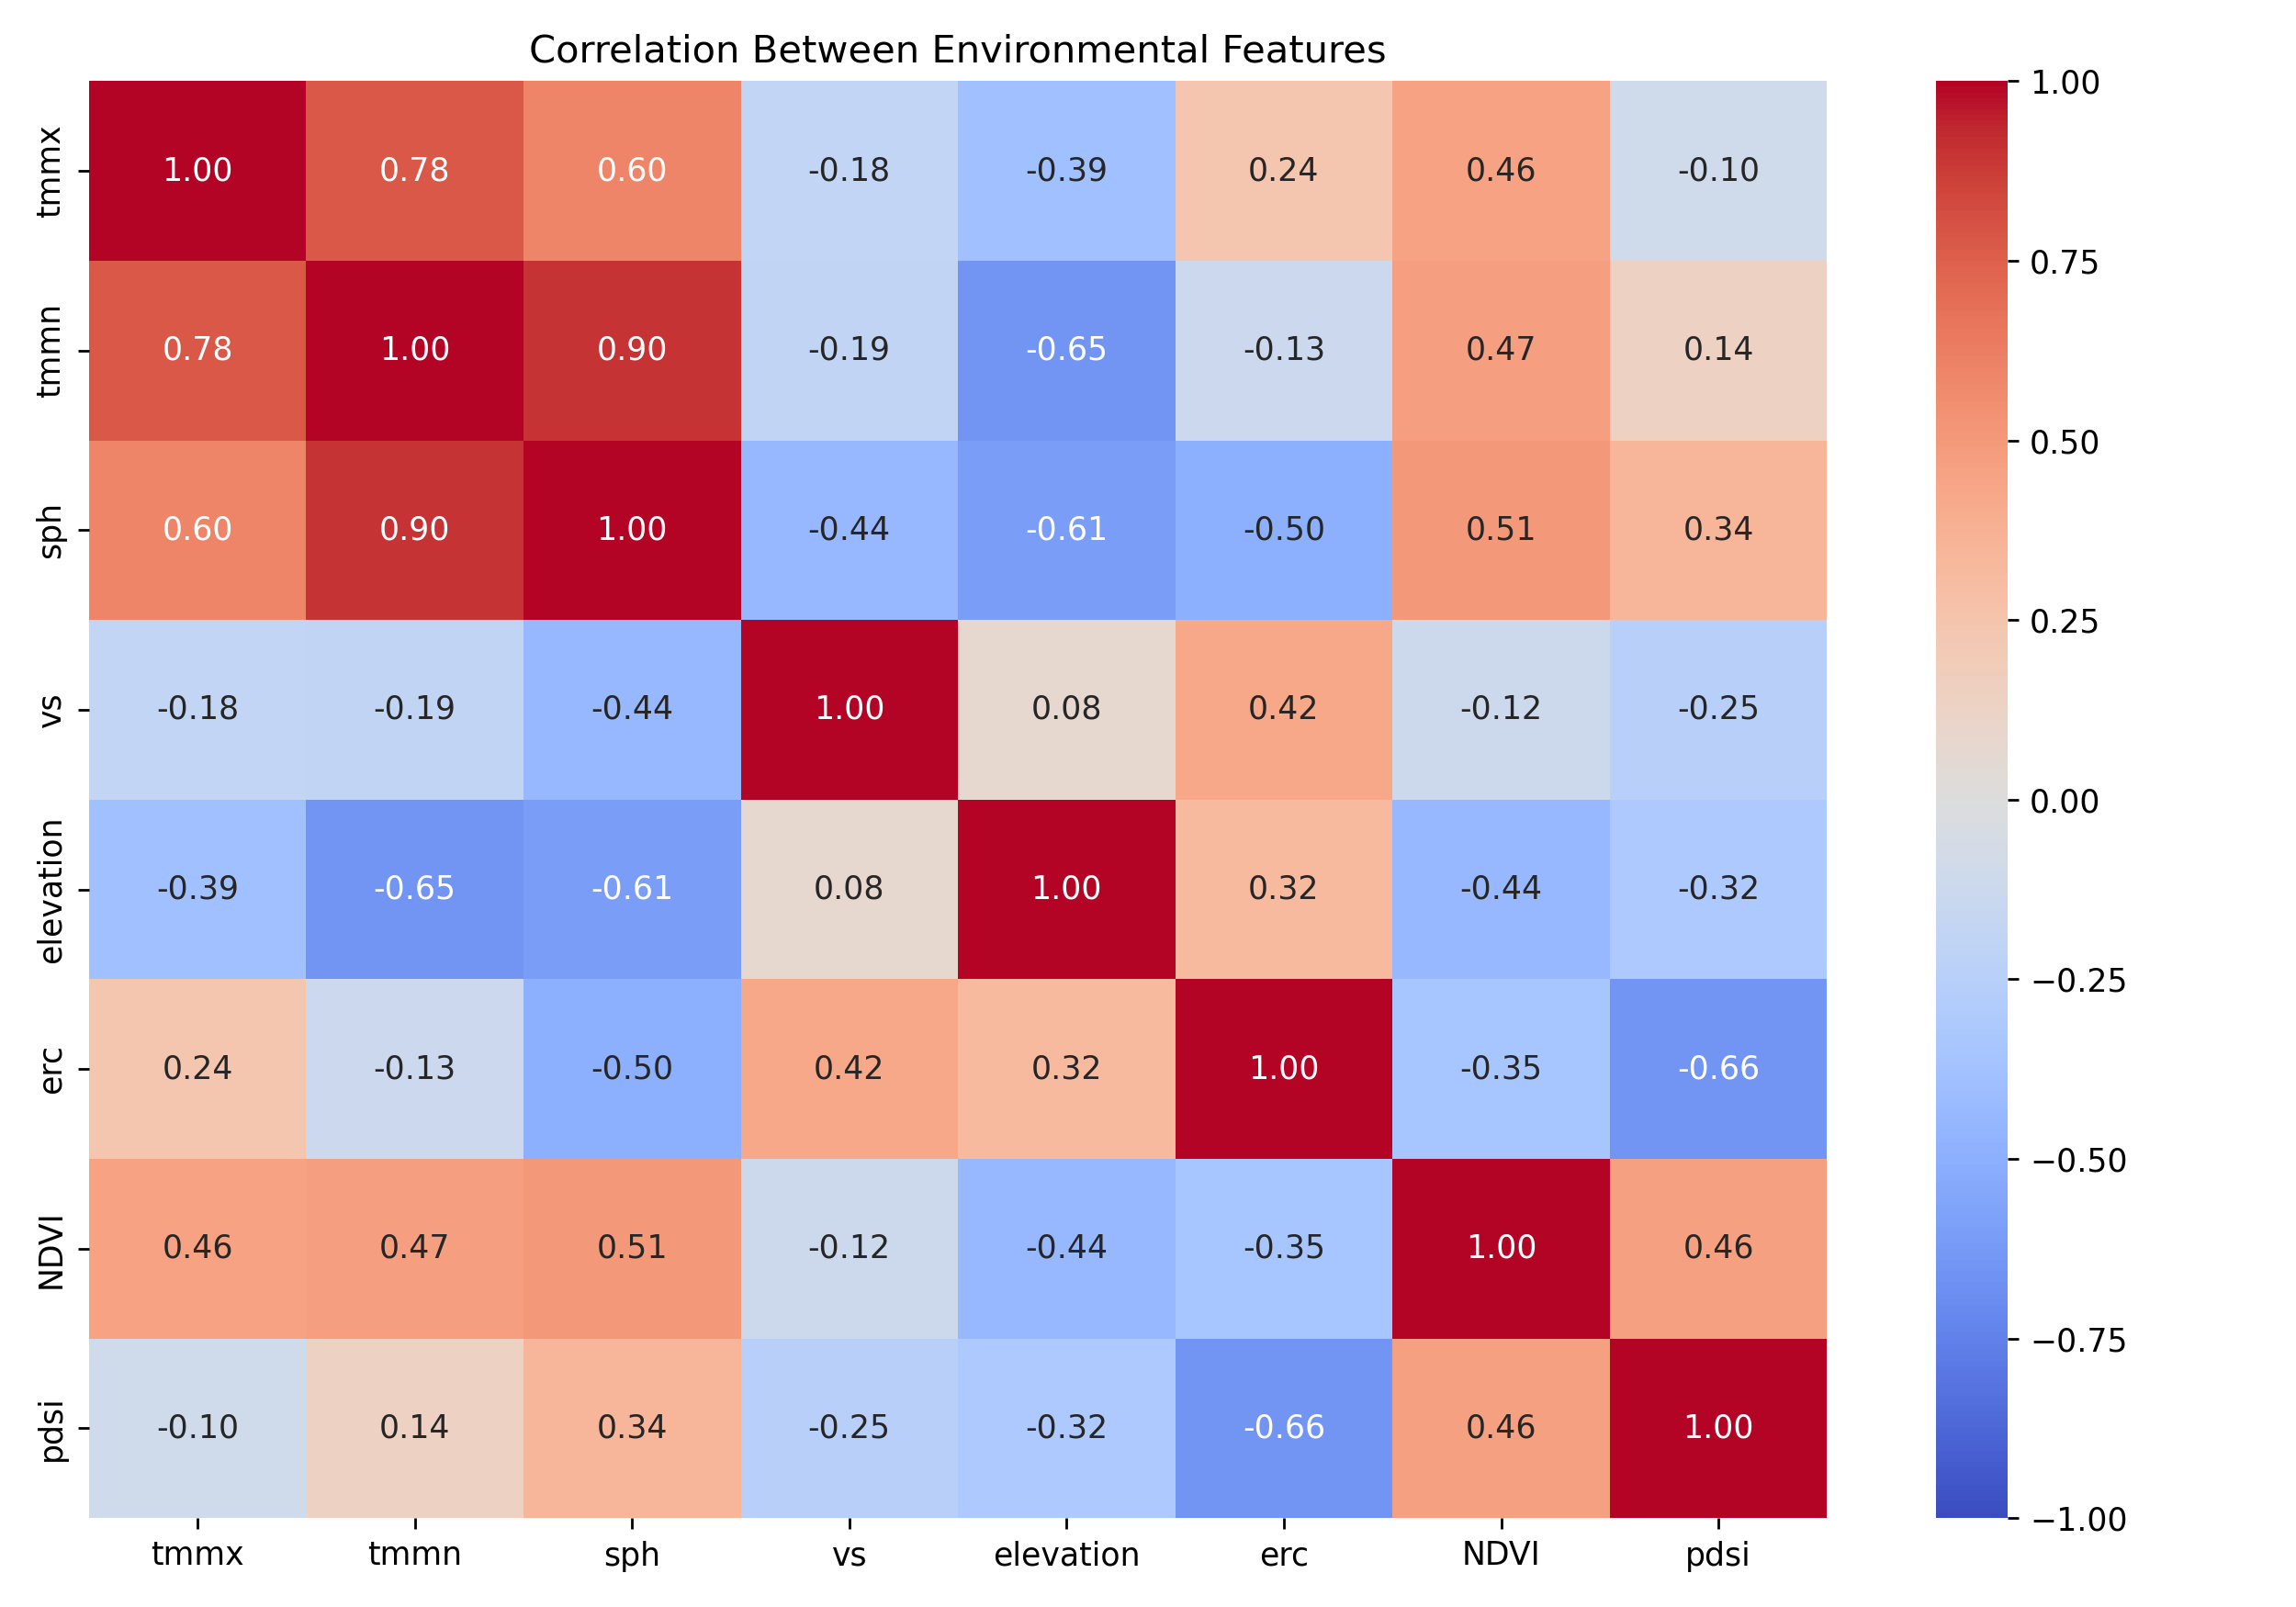
\includegraphics[width=0.95\columnwidth]{correlation_heatmap.png}
\caption{Cross-feature Pearson correlation heatmap demonstrating physical consistency among environmental channels.}
\label{fig:corr}
\end{figure}

\subsection{Linear Correlation with the Target ($FireMask$)}
We examined the linear correlation of each individual feature with next-day fire spread across splits:
\begin{itemize}
    \item $\texttt{PrevFireMask}$: $r = +0.12$ on train and $r = +0.31$ on test. Antecedent fire state represents the sole raw variable displaying strong, consistent target correlation across splits.
    \item Atmospheric and Weather Features: All 11 raw environmental and weather channels display $|r| \le 0.015$ on the training split.
\end{itemize}

\begin{figure}[H]
\centering
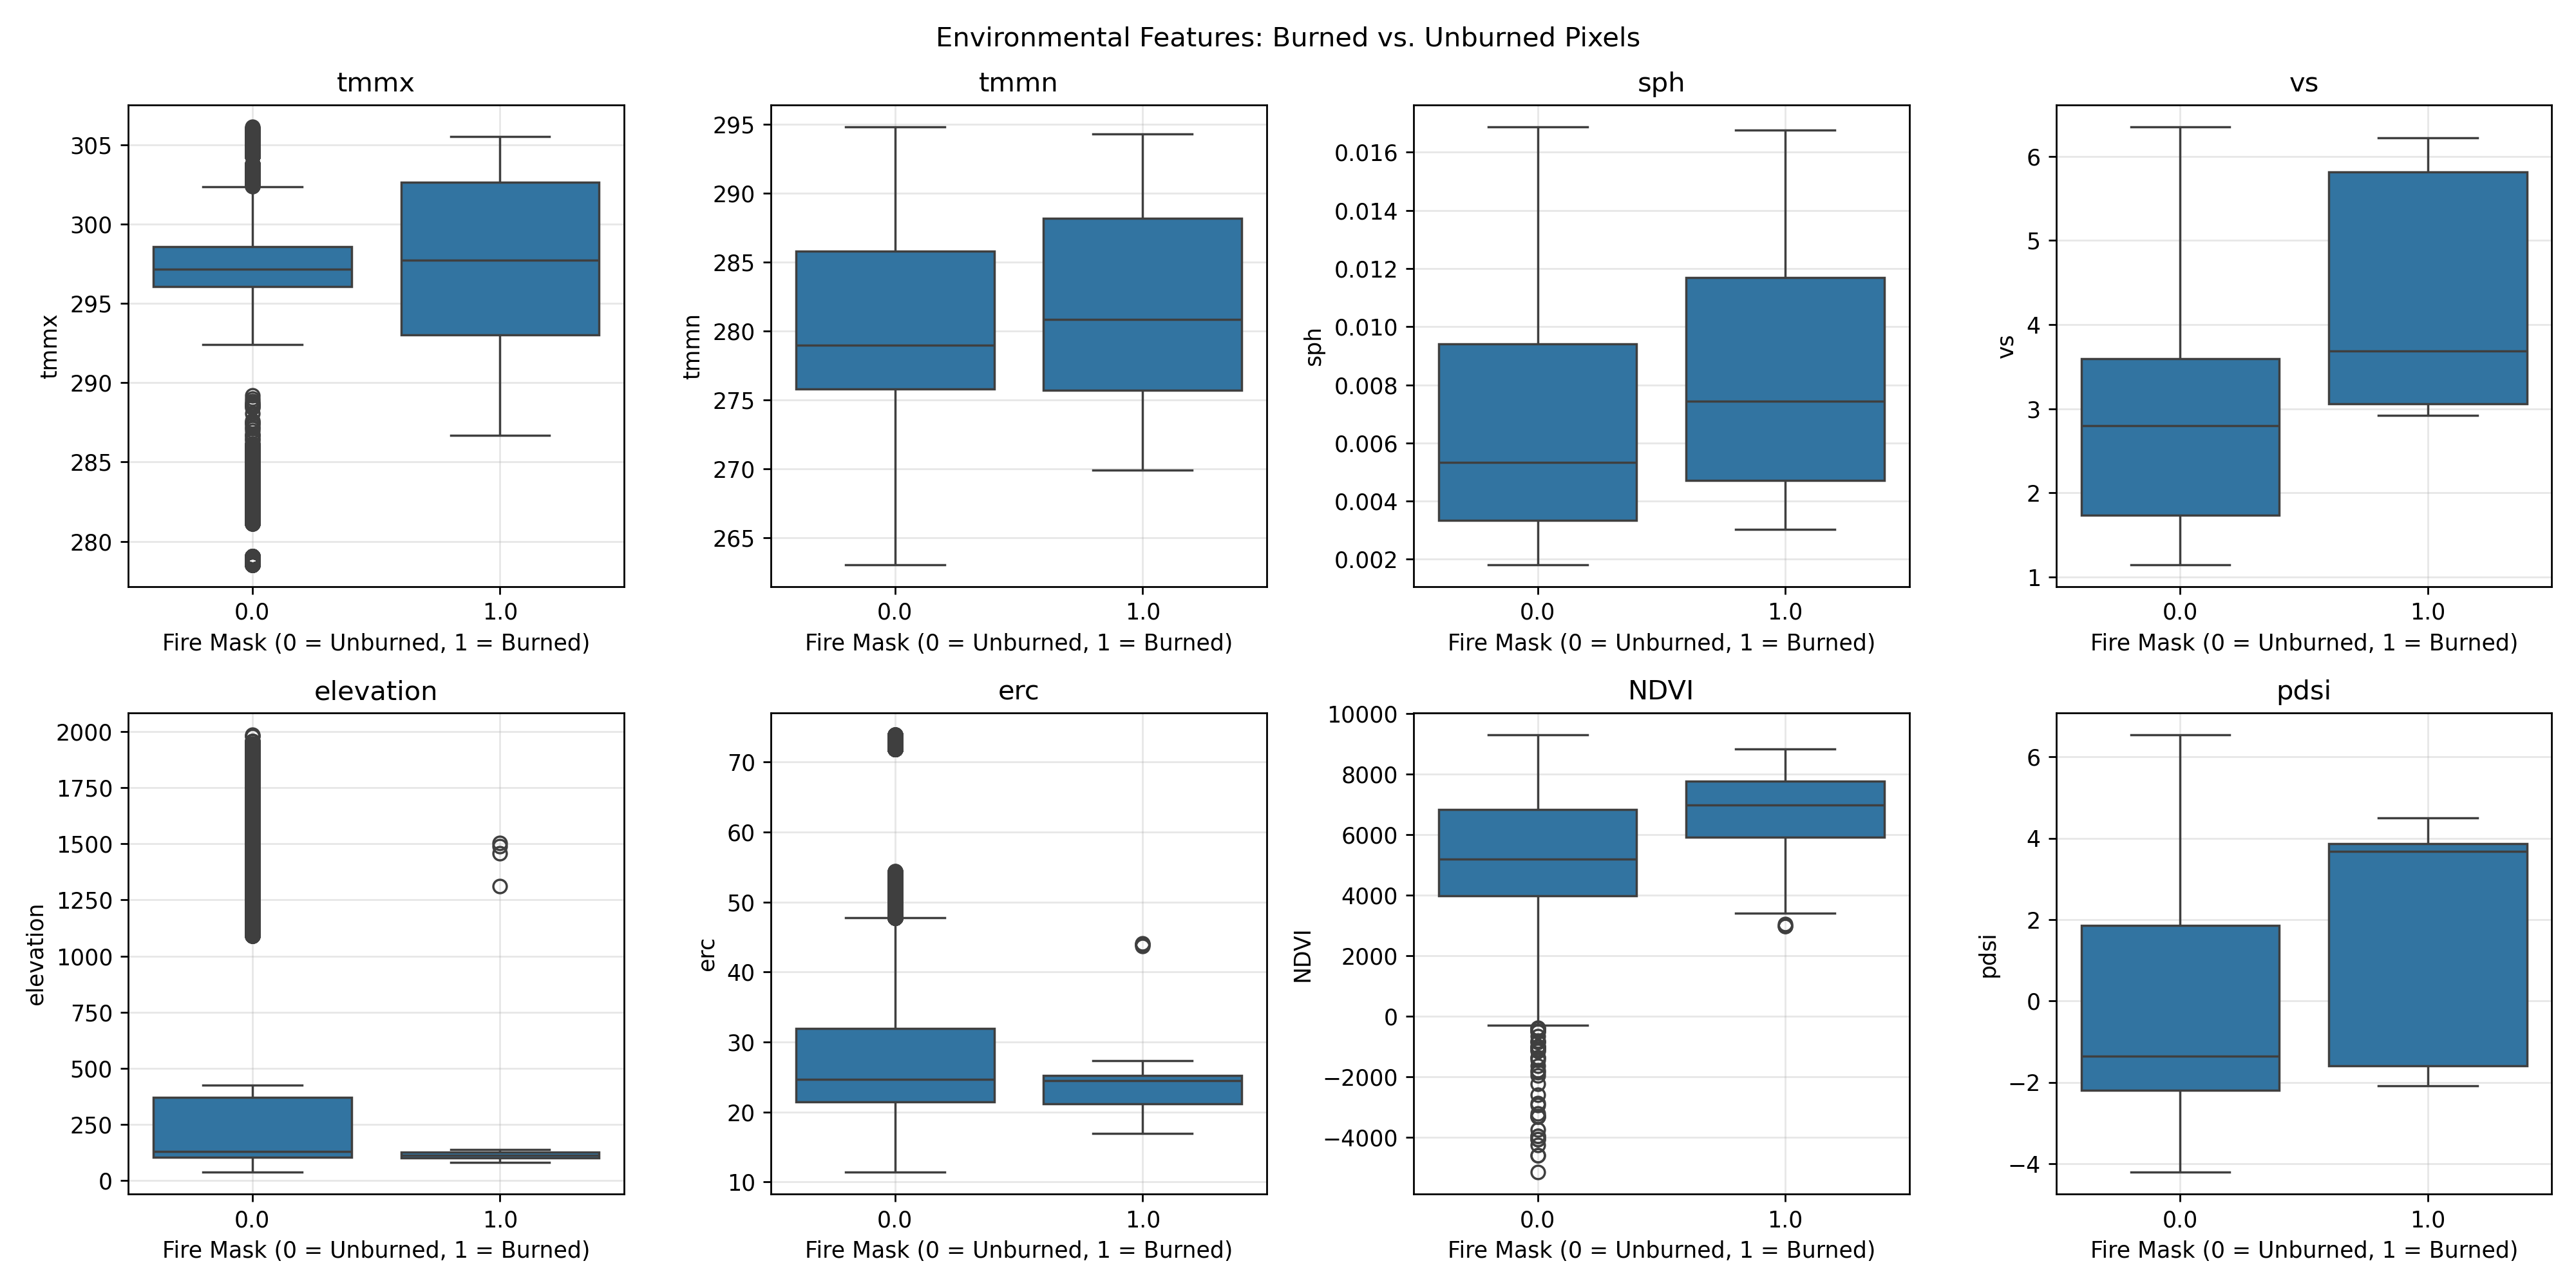
\includegraphics[width=0.95\columnwidth]{burned_vs_unburned.png}
\caption{Distributions of primary environmental features stratified by next-day burned vs. unburned status.}
\label{fig:burned_vs_unburned}
\end{figure}

\section{Feature Engineering and Domain Indicators}
To enhance model expressiveness beyond raw sensor measurements, we design five domain-engineered features based on combustion physics and spatial interaction principles:

\begin{enumerate}
    \item \textbf{Diurnal Temperature Range ($\texttt{temp\_range}$)}:
    \begin{equation}
        \Delta T = tmmx - tmmn
    \end{equation}
    Elevated temperature fluctuations reflect low atmospheric relative humidity and cloudless radiative heating, which desiccate combustible ground fuels.
    
    \item \textbf{Decomposed Wind Vector Components ($\texttt{wind\_u}, \texttt{wind\_v}$)}:
    Direct angular direction $th \in [0^\circ, 360^\circ]$ introduces an artificial numerical discontinuity ($359^\circ \approx 1^\circ$). We decompose wind into orthogonal Cartesian components:
    \begin{equation}
        u_{\text{wind}} = vs \cdot \sin\left(\frac{\pi \cdot th}{180}\right), \quad v_{\text{wind}} = vs \cdot \cos\left(\frac{\pi \cdot th}{180}\right)
    \end{equation}
    
    \item \textbf{Composite Drought-Fuel Flammability Index ($\texttt{drought\_fuel\_index}$)}:
    Couples acute fuel moisture with chronic regional hydrological deficit:
    \begin{equation}
        \text{DFI} = erc \cdot (pdsi + 1.0)
    \end{equation}
    
    \item \textbf{Spatial Neighborhood Combustion Convolutions}:
    Wildfires spread via contiguous convective and radiative heat transfer to neighboring cells. Using 2D spatial convolution kernels over the antecedent fire mask $\texttt{PrevFireMask}$, we compute the count of actively burning neighbors in the local Moore neighborhood ($3 \times 3$, 8 adjacent cells) and extended neighborhood ($5 \times 5$, 24 adjacent cells):
    \begin{equation}
        \text{Neighbor}_{3\times 3}(i, j) = \sum_{a=-1}^{1} \sum_{b=-1}^{1} \texttt{PrevFireMask}(i+a, j+b) - \texttt{PrevFireMask}(i, j)
    \end{equation}
\end{enumerate}

The spatial neighbor feature exhibits outstanding discriminative power: non-fire pixels average 0.01 burning neighbors, whereas next-day fire pixels average \textbf{0.935 burning neighbors} ($93.5\times$ increase). The correlation of this feature with $\texttt{FireMask}$ reaches $r = +0.15$ on train and $r = +0.37$ on test, outperforming every raw feature.

\begin{figure}[H]
\centering
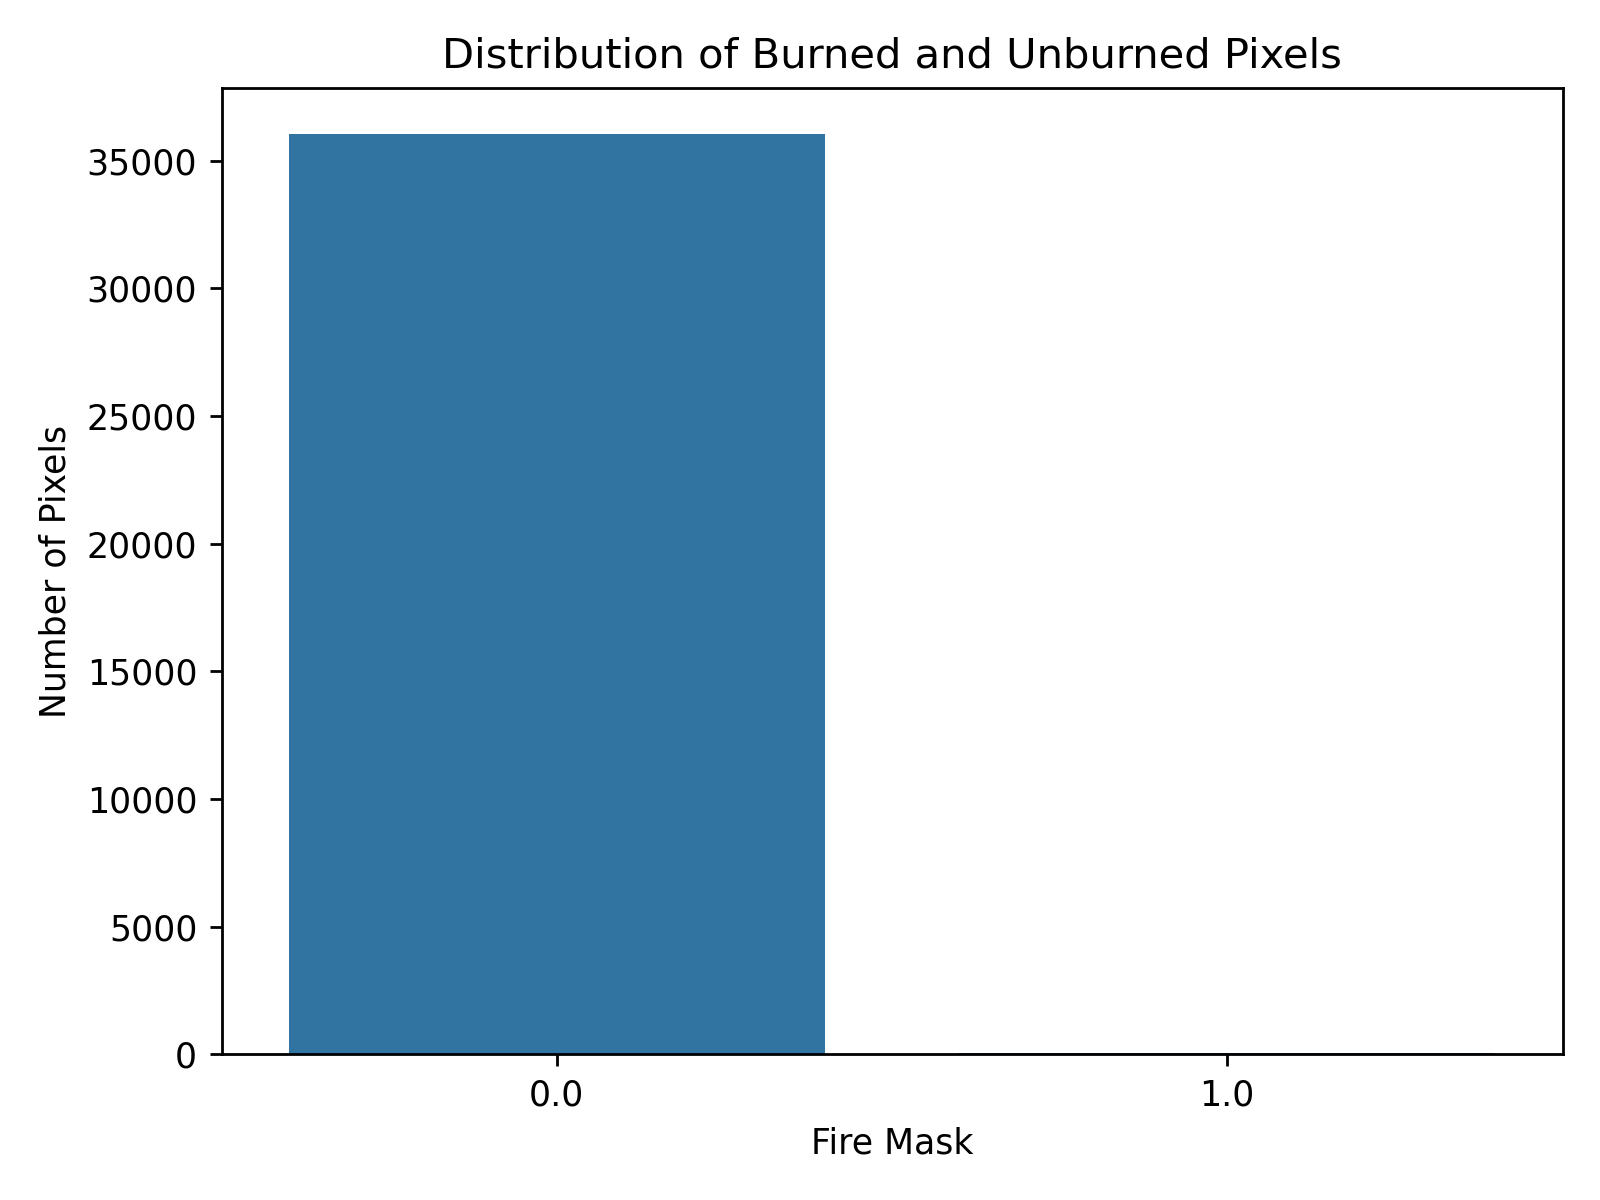
\includegraphics[width=0.95\columnwidth]{fire_mask_distribution.png}
\caption{Extreme target class imbalance depicted across positive fire pixels ($y=1$) and negative pixels ($y=0$).}
\label{fig:fire_dist}
\end{figure}

\subsection{Feature Ablation Groups}
To quantify the incremental value of each information category, we structure four cumulative feature groups:
\begin{itemize}
    \item \textbf{Group A (Weather, $K=6$)}: $th, vs, tmmn, tmmx, sph, pr$.
    \item \textbf{Group B ($K=7$)}: Group A $+$ $\texttt{PrevFireMask}$.
    \item \textbf{Group C ($K=12$)}: Group B $+$ $elevation, pdsi, NDVI, population, erc$.
    \item \textbf{Group D ($K=18$)}: Group C $+$ $\texttt{temp\_range}, u_{\text{wind}}, v_{\text{wind}}, \text{DFI}, \text{Neighbor}_{3\times 3}, \text{Neighbor}_{5\times 5}$.
\end{itemize}

\section{Machine Learning Models and Rare-Event Evaluation}

\subsection{Candidate Model Architectures}
We deploy four distinct classification paradigms:
\begin{enumerate}
    \item \textbf{Persistence Baseline}: A zero-learning operational heuristic predicting that tomorrow's fire state matches today's: $\hat{y}_{i, t+1} = \texttt{PrevFireMask}_{i, t}$.
    \item \textbf{Logistic Regression}: Regularized generalized linear model with class reweighting (\texttt{class\_weight='balanced'}):
    \begin{equation}
        P(y=1|\mathbf{x}) = \sigma(\mathbf{w}^T \mathbf{x} + b)
    \end{equation}
    \item \textbf{LightGBM}: Fast, histogram-based gradient boosted decision tree ensemble with leaf-wise tree growth~\cite{ke2017lightgbm}, configured with cost-sensitive weighting ($\texttt{scale\_pos\_weight} = 8$).
    \item \textbf{XGBoost}: Depth-wise gradient boosted decision tree algorithm~\cite{chen2016xgboost} utilizing second-order gradient approximations and identical cost-sensitive scaling ($\texttt{scale\_pos\_weight} = 8$).
\end{enumerate}

\subsection{Evaluation Metrics for Severe Imbalance}
In extreme rare-event regimes, standard accuracy is non-informative: predicting $y=0$ everywhere yields $98.91\%$ accuracy while failing completely. We evaluate with specialized rare-event metrics:
\begin{itemize}
    \item \textbf{PR-AUC (Average Precision)}: Computes the area under the Precision-Recall curve. As established by Saito and Rehmsmeier~\cite{saito2015precision}, PR-AUC evaluates true positive recovery without being distorted by immense true negative volumes. The baseline score for an uninformative random classifier equals the positive class prevalence $\pi$ (e.g., $0.0015$ on validation, $0.0109$ on test).
    \item \textbf{ROC-AUC}: Measures ranking capability across all thresholds ($0.50$ indicates random chance; $1.0$ indicates perfect ranking).
    \item \textbf{Recall @ Fixed 5\% False Positive Rate (FPR)}: Measures operational safety: if disaster responders tolerate flagging $5\%$ of unburned land as false alarms, what percentage of genuine wildfires are intercepted?
    \item \textbf{Validation-Tuned Decision Threshold ($\tau^*$)}: The default threshold $\tau=0.5$ fails in rare-event settings. We optimize $\tau^*$ strictly on validation predictions by maximizing the F1-score:
    \begin{equation}
        \tau^* = \arg\max_{\tau} F_1(\tau) = \arg\max_{\tau} \frac{2 \cdot P(\tau) \cdot R(\tau)}{P(\tau) + R(\tau)}
    \end{equation}
\end{itemize}

\section{Empirical Results and Benchmark Evaluation}

\subsection{Validation Benchmark Comparison}
Table~\ref{tab:val_comparison} presents the empirical benchmark across all evaluated architectures on the validation partition ($N=26,125$, 39 positive fires).

\begin{table}[H]
\centering
\caption{Consolidated Validation Benchmark Performance Across Models (Group D Features).}
\label{tab:val_comparison}
\begin{tabular}{lccc}
\toprule
\textbf{Model Architecture} & \textbf{PR-AUC} & \textbf{ROC-AUC} & \textbf{Recall @ 5\% FPR} \\
\midrule
Persistence Baseline & 0.00149 & 0.4983 & 0.0000 \\
Logistic Regression & 0.00084 & 0.1414 & 0.0000 \\
\textbf{LightGBM} & \textbf{0.00159} & \textbf{0.5175} & \textbf{0.0000} \\
XGBoost & 0.00091 & 0.1989 & 0.0000 \\
\midrule
Random Baseline ($\pi$) & 0.00149 & 0.5000 & 0.0500 \\
\bottomrule
\end{tabular}
\end{table}

LightGBM was the sole trained model to achieve an ROC-AUC above the $0.50$ random threshold ($0.5175$) and nominally surpassed the random PR-AUC baseline ($0.00159$ vs. $0.00149$). Both Logistic Regression and XGBoost scored substantially below $0.50$ ROC-AUC. 

This phenomenon occurred because in the validation partition, all 39 active fires occurred in locations that were unburned on day $t$, while all 88 pixels that burned on day $t$ extinguished on day $t+1$. Having learned from training that ``burning today implies burning tomorrow'', these models inverted rankings on this specific validation patch. LightGBM was selected as our representative model for held-out testing.

\subsection{Feature Group Ablation Study}
We conducted an ablation study across Feature Groups A through D using LightGBM on the validation set, summarized in Table~\ref{tab:ablation}.

\begin{table}[H]
\centering
\caption{LightGBM Feature Group Ablation on the Validation Set.}
\label{tab:ablation}
\begin{tabular}{lccc}
\toprule
\textbf{Feature Group} & \textbf{Num Features} & \textbf{PR-AUC} & \textbf{ROC-AUC} \\
\midrule
Group A (Weather) & 6 & 0.0016 & 0.30 \\
Group B ($+$ Fire Mask) & 7 & 0.0019 & 0.55 \\
Group C ($+$ Topo/Fuel/Pop) & 12 & \textbf{0.0022} & \textbf{0.66} \\
Group D ($+$ Engineered/Spatial) & 18 & 0.0016 & 0.50 \\
\bottomrule
\end{tabular}
\end{table}

While ROC-AUC increases from $0.30$ to $0.66$ through Group C, PR-AUC remains essentially bounded by the random baseline rate across all groups. With only 39 positive fire events in validation, ROC fluctuations primarily reflect sample variance on a single fire event.

\subsection{Held-Out Test Set Results}
The final model (LightGBM on Group D) was deployed to the held-out test partition ($N=14,429$, 157 positive fires). Results are documented in Table~\ref{tab:test_results}.

\begin{table}[H]
\centering
\caption{Held-Out Test Set Evaluation: LightGBM vs. Uninformative Baselines.}
\label{tab:test_results}
\begin{tabular}{lcc}
\toprule
\textbf{Evaluation Metric} & \textbf{Trained LightGBM} & \textbf{Random Baseline} \\
\midrule
PR-AUC (Average Precision) & 0.0109 & 0.0109 \\
ROC-AUC & 0.4998 & 0.5000 \\
Recall @ 5\% False Alarm Rate & 0.0000 & 0.0500 \\
Overall Classification Accuracy & 98.88\% & 98.91\% \\
\bottomrule
\end{tabular}
\end{table}

Applying the validation-optimized decision threshold ($\tau^* = 0.0007$) yielded the $2 \times 2$ test confusion matrix in Table~\ref{tab:confusion_matrix}.

\begin{table}[H]
\centering
\caption{Held-Out Test Set Confusion Matrix ($\tau^* = 0.0007$).}
\label{tab:confusion_matrix}
\begin{tabular}{lcc}
\toprule
& \textbf{Ground Truth Fire} & \textbf{Ground Truth No-Fire} \\
\midrule
\textbf{Model Predicted Fire} & 0 (True Positive) & 4 (False Positive) \\
\textbf{Model Predicted No-Fire} & 157 (False Negative) & 14,268 (True Negative) \\
\bottomrule
\end{tabular}
\end{table}

The trained LightGBM model captured \textbf{0 out of 157} real fire pixels, generating 4 false alarms and 157 false negatives. Despite achieving $98.88\%$ accuracy, the model was completely ineffective operationally.

\section{Diagnostic Analysis and Key Insights}

\subsection{The Heuristic vs. Learned Model Paradox}
To ascertain whether the predictive failure stemmed from uninformative features or model training collapse, we evaluated simple zero-parameter heuristics on the exact same held-out test set, as reported in Table~\ref{tab:heuristics}.

\begin{table}[H]
\centering
\caption{Zero-Parameter Spatial Heuristics vs. Trained GBDT on Held-Out Test Data.}
\label{tab:heuristics}
\begin{tabularx}{\columnwidth}{lXcc}
\toprule
\textbf{Prediction Method} & \textbf{Underlying Mechanism} & \textbf{PR-AUC} & \textbf{Gain vs Random} \\
\midrule
Random Baseline & Uninformative uniform guessing & 0.011 & $1.0\times$ \\
Trained LightGBM & GBDT on 18 tabular features & 0.011 & $1.0\times$ \\
Persistence Rule & Predict fire if $\texttt{PrevFireMask}=1$ & 0.109 & $10.0\times$ \\
\textbf{Neighbor Count Rule} & \textbf{Predict fire by $\text{Neighbor}_{3\times 3}$ count} & \textbf{0.182} & \textbf{16.7}$\times$ \\
\bottomrule
\end{tabularx}
\end{table}

This comparison provides a striking insight: \textbf{strong predictive signal exists in the spatial features, but the tree-based machine learning model failed to learn it.} A simple heuristic based on our engineered spatial neighbor count achieves a PR-AUC of \textbf{0.182} ($17\times$ higher than the trained model).

\subsection{Root Causes of Model Collapse}
We identify three primary drivers of the tabular GBDT failure:
\begin{enumerate}
    \item \textbf{Extreme Training Positive Sparsity ($N=62$)}: Across 77,244 training instances, the model observed only 62 positive fire pixels. GBDT splitting criteria struggled to partition statistically robust leaf nodes. Consequently, the test predictions collapsed into only 3 discrete output probabilities across all 14,429 test instances.
    \item \textbf{Threshold Transferability Breakdown}: The operational decision threshold ($\tau^* = 0.0007$) selected on the validation model from Notebook~05 failed to transfer to the retrained LightGBM checkpoint in Notebook~06, illustrating the hazard of transferring uncalibrated rare-event cutoffs.
    \item \textbf{Dominance of Spatial Autocorrelation over Weather}: Meteorological variables exhibited near-zero correlation with fire spread ($|r| \le 0.015$), whereas spatial neighbor counts reached $r = 0.37$. Tabular tree models without explicit 2D spatial awareness treat spatial neighbor counts as isolated scalars rather than coherent geometric fire perimeters.
\end{enumerate}

\begin{figure}[H]
\centering
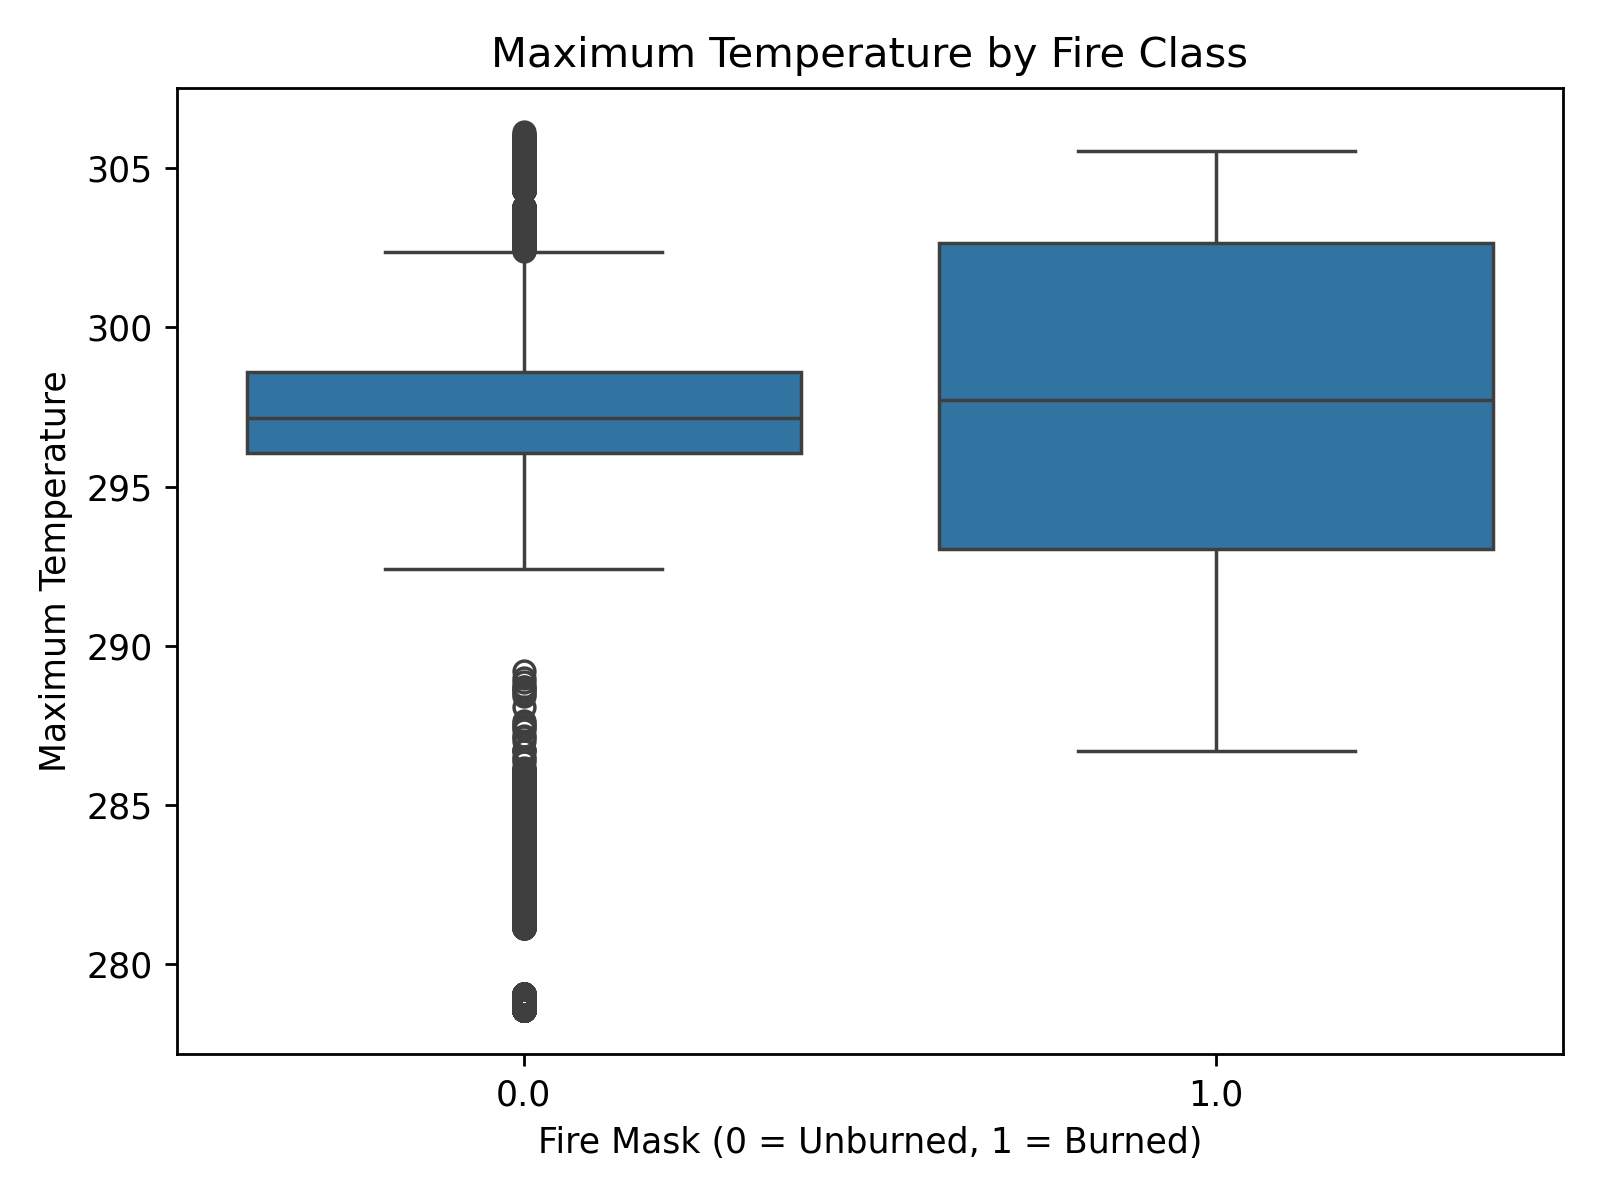
\includegraphics[width=0.95\columnwidth]{temperature_by_fire_class.png}
\caption{Maximum temperature ($tmmx$) distributions stratified by fire presence, illustrating minimal separable margin in scalar weather features.}
\label{fig:temp_by_class}
\end{figure}

\section{Pipeline Auditing and Methodological Corrections}
During pipeline verification, we identified and corrected four critical bugs to guarantee empirical integrity:
\begin{enumerate}
    \item \textbf{Spatial Convolution Pre-Subsampling Calculation}: Initially, spatial neighbor counts were computed \textit{after} negative subsampling, which eliminated real neighboring fire pixels and collapsed neighbor counts to near zero. We corrected the pipeline to compute 2D neighbor convolutions on the complete $64 \times 64$ patch grid prior to row sampling. This correction increased the train correlation $r$ with $\texttt{FireMask}$ from $+0.065$ to $+0.154$.
    \item \textbf{Patch Identifier Disambiguation}: Previously, maps across different splits shared identical zero-indexed integer IDs, corrupting cross-split overlap verification. We prepended partition names to IDs (e.g., $\texttt{train\_0}$, $\texttt{test\_0}$).
    \item \textbf{Boolean Assertion in Leakage Validator}: The leakage checking script contained a bug that printed \texttt{[PASS]} unconditionally regardless of assertion status. We refactored the validator to enforce strict boolean evaluations.
    \item \textbf{Quantitative Metric Reconciliation}: Corrected narrative metric references across notebooks to ensure all figures match verified experimental logs.
\end{enumerate}

\section{Limitations}
\begin{itemize}
    \item \textbf{Sample Size Constraints}: Utilizing 30 train, 10 validation, and 10 test patches provided only 62 training fire pixels, limiting statistical learning capacity.
    \item \textbf{Validation Clustering}: All validation fire events occurred within a single patch, making validation ranking metrics sensitive to local fire dynamics.
    \item \textbf{Tabular Coordinate Loss}: Flattening 2D spatial patches into 1D tabular rows discards essential spatial geometry, including fire line shape, front curvature, and atmospheric wind advection.
    \item \textbf{Coarse Weather Resolution}: ERA5 reanalysis data ($31\text{ km}$ native resolution) is bilinearly interpolated onto a $1\text{ km}$ grid, creating smooth gradients that cannot distinguish adjacent pixels.
\end{itemize}

\section{Roadmap and Phase 2 Next Steps}
Building directly upon these Phase~1 findings, the Phase~2 roadmap focuses on:
\begin{enumerate}
    \item \textbf{Multi-Shard Ingestion}: Scaling data extraction to hundreds of TFRecord patches to increase positive fire events from $N=62$ to thousands of instances.
    \item \textbf{Regularized GBDT Tuning}: Enforcing aggressive leaf regularization ($\texttt{min\_child\_samples} \ge 20$) and early stopping monitored directly on PR-AUC.
    \item \textbf{2D Spatial Deep Learning (U-Net)}: Transitioning from tabular pixel models to fully convolutional 2D U-Net neural architectures~\cite{ronneberger2015unet}. Looking at the full $64 \times 64$ field of view allows the network to natively learn spatial fire perimeter expansion, advection, and topological barrier constraints.
\end{enumerate}

\section{Team Roles and Workload Contributions}
All experimental outputs, figures, and pipeline steps reflect collaborative execution across Team TensorTitans (Section C) as documented in Table~\ref{tab:contributions}.

\begin{table}[H]
\centering
\caption{Team Member Roles and Deliverable Ownership.}
\label{tab:contributions}
\begin{tabularx}{\columnwidth}{lX}
\toprule
\textbf{Team Member} & \textbf{Primary Contributions and Deliverables} \\
\midrule
\textbf{Vanshika} & Literature review, TFRecord ingestion architecture, raw geospatial schema audit, \texttt{src/data\_loader.py}. \\
\textbf{Riya / Tejas} & Exploratory data analysis, multi-channel visualization heatmaps, Phase~1 research reporting. \\
\textbf{Krish} & Spatial neighbor convolutions, feature engineering, model training (GBDTs), diagnostic error analysis. \\
\textbf{Nitanshu} & Leakage-safe split validator, threshold optimization, rare-event metrics, pipeline reproducibility verification. \\
\bottomrule
\end{tabularx}
\end{table}

\section{Glossary of Machine Learning and Wildfire Terminology}
Table~\ref{tab:glossary} provides concise definitions of key domain and machine learning terms used throughout this study.

\begin{table}[H]
\centering
\caption{Glossary of Core Machine Learning and Wildfire Concepts.}
\label{tab:glossary}
\begin{tabularx}{\columnwidth}{lX}
\toprule
\textbf{Concept} & \textbf{Technical Definition} \\
\midrule
\textbf{Grid Pixel} & A $1\text{ km} \times 1\text{ km}$ land parcel represented as a single tabular sample instance. \\
\textbf{Target Label} & Binary indicator ($\texttt{FireMask} \in \{0, 1\}$) of active thermal detection on day $t+1$. \\
\textbf{Data Leakage} & Spurious inflation of model performance caused by evaluation samples sharing information with training data. \\
\textbf{PR-AUC} & Area under the Precision-Recall curve; the primary metric for rare-event imbalance evaluation. \\
\textbf{ROC-AUC} & Area under the Receiver Operating Characteristic curve; measures ranking quality ($0.5$ is random). \\
\textbf{Operating Threshold} & Decision boundary $\tau \in [0, 1]$ above which model probabilities are classified as active fire. \\
\bottomrule
\end{tabularx}
\end{table}

\section{Conclusion}
Phase~1 of this project established a rigorous, leakage-free benchmark for next-day wildfire spread prediction. Our empirical findings demonstrate that extreme class imbalance ($< 1.1\%$) and spatial autocorrelation govern this domain. While scalar tabular GBDT models collapsed under severe positive sparsity ($N=62$), our spatial neighbor convolution feature demonstrated that strong spatial signals exist in antecedent thermal data ($17\times$ above random guessing). This definitive finding directly motivates and justifies the transition to 2D spatial deep learning (U-Net) in Phase~2.

\bibliographystyle{IEEEtran}
\bibliography{references}

\end{document}
